\documentclass[tikz,border=8pt]{standalone}
% Shared look for every TikZ diagram. Load with \input{../../tools/tikz-style.tex}
\usepackage[T1]{fontenc}
\usepackage{lmodern}
\renewcommand{\sfdefault}{lmr}  % diagrams use the same serif as the text
\usetikzlibrary{arrows.meta, positioning, shapes.geometric, calc, fit, backgrounds}
\definecolor{cblue}{HTML}{4C78A8}
\definecolor{corange}{HTML}{F58518}
\definecolor{cgreen}{HTML}{54A24B}
\definecolor{cred}{HTML}{E45756}
\definecolor{cpurple}{HTML}{B279A2}
\definecolor{cgrey}{HTML}{6B6B6B}
\tikzset{
  every picture/.style={font=\sffamily, line width=1.2pt},
  box/.style={draw=#1, fill=#1!12, rounded corners=4pt, align=center, inner sep=7pt, minimum height=1.1cm},
  box/.default=cgrey,
  arrow/.style={-{Stealth[length=3mm]}, draw=cgrey, line width=1.4pt},
  title/.style={font=\sffamily\bfseries\Large},
  note/.style={font=\sffamily\small, text=cgrey, align=center},
}
\AtBeginDocument{\hyphenpenalty=10000 \exhyphenpenalty=10000}

\begin{document}
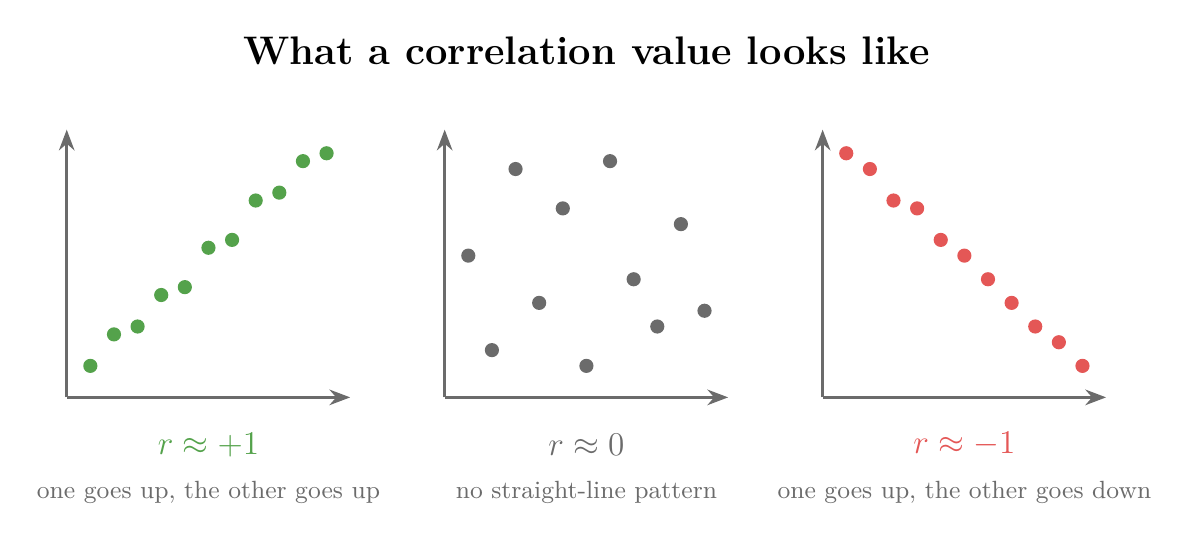
\begin{tikzpicture}
  \node[title] at (6.6,4.4) {What a correlation value looks like};
  % one panel: #1 x-offset, #2 colour, #3 point list, #4 label, #5 sub-label
  \newcommand{\panel}[5]{
    \begin{scope}[xshift=#1cm]
      \draw[cgrey, line width=1pt, -{Stealth}] (0,0) -- (3.6,0);
      \draw[cgrey, line width=1pt, -{Stealth}] (0,0) -- (0,3.4);
      \foreach \x/\y in {#3} \fill[#2] (\x,\y) circle (0.09);
      \node[font=\large\bfseries, text=#2] at (1.8,-0.6) {#4};
      \node[note] at (1.8,-1.2) {#5};
    \end{scope}}
  \panel{0}{cgreen}{0.3/0.4, 0.6/0.8, 0.9/0.9, 1.2/1.3, 1.5/1.4, 1.8/1.9, 2.1/2.0, 2.4/2.5, 2.7/2.6, 3.0/3.0, 3.3/3.1}
        {$r \approx +1$}{one goes up, the other goes up}
  \panel{4.8}{cgrey}{0.3/1.8, 0.6/0.6, 0.9/2.9, 1.2/1.2, 1.5/2.4, 1.8/0.4, 2.1/3.0, 2.4/1.5, 2.7/0.9, 3.0/2.2, 3.3/1.1}
        {$r \approx 0$}{no straight-line pattern}
  \panel{9.6}{cred}{0.3/3.1, 0.6/2.9, 0.9/2.5, 1.2/2.4, 1.5/2.0, 1.8/1.8, 2.1/1.5, 2.4/1.2, 2.7/0.9, 3.0/0.7, 3.3/0.4}
        {$r \approx -1$}{one goes up, the other goes down}
\end{tikzpicture}
\end{document}
